\documentclass[11pt,a4paper]{article}
\usepackage[hyperref]{acl2017}
\usepackage{times}
\usepackage{latexsym}

\usepackage{url}
\usepackage{booktabs}
\usepackage{graphicx}

%\aclfinalcopy % Uncomment this line for the final submission
%\def\aclpaperid{***} %  Enter the acl Paper ID here

%\setlength\titlebox{5cm}
% You can expand the titlebox if you need extra space
% to show all the authors. Please do not make the titlebox
% smaller than 5cm (the original size); we will check this
% in the camera-ready version and ask you to change it back.

\newcommand\BibTeX{B{\sc ib}\TeX}

\title{Toward a Comparable Corpora of Latvian, Russian and English Tweets}

\author{First Author \\
  Affiliation / Address line 1 \\
  Affiliation / Address line 2 \\
  Affiliation / Address line 3 \\
  {\tt email@domain} \\\And
  Second Author \\
  Affiliation / Address line 1 \\
  Affiliation / Address line 2 \\
  Affiliation / Address line 3 \\
  {\tt email@domain} \\}

\date{}

\begin{document}
\maketitle

\begin{abstract}
Twitter has become a rich source for linguistic data. Here, a possibility of building a trilingual Latvian-Russian-English corpus of tweets from Riga, Latvia is investigated. Such a corpus, once constructed, might be of great use for multiple purposes such as training machine translation models, examining cross-lingual phenomena and studying the population of Riga. This pilot study shows that it is feasible to build such a resource. The resulting corpus is made publicly available and can be used to construct a large comparable corpus.
\end{abstract}

\section{Introduction}
\label{sec:introduction}

Comparable corpora are widely used by the natural language processing community to build machine translation or information retrieval models. The goal of this work is to investigate whether it is possible to build a comparable linguistic resource of tweets that originates from one specific location--Riga, Latvia. Riga is a great location for this because it is a multilingual city in which Latvian and Russian are both widely used in everyday life, and English is used a lingua franca in tourism and commerce.

Despite the fact that Latvian and Russian are widely used, there is little interaction between the two ethnic communities. The local media consists of two subsystems (Latvian and Russian) which use different sources and present different views on current affairs \cite{muiznieks2010}. However, despite the fact that large media portals tend to have separate Latvian and Russian web-sites, the same opinions are found in comments to controversial content on both versions of web-sites, making the Internet a public space for a dialogue  between the ethnic communities \cite{sulmane2010}. The resulting corpus of user generated content is a fruitful resource for studying the integration of the two communities, by identifying what is being discussed; how, and most importantly why it is being discussed.

% Twitter,\footnote{\url{https://twitter.com}} a microblog platform, is used as the data source in this pilot study. Over the period of 5 months (November 2016 to March 2017), tweets from Riga were collected, filtered and analysed. The main goal of the analysis is to investigate whether a creation of a comparable tweet corpus is feasible and what the corpus construction strategy should be.

The analysis of the tweets, shows that some real world events, such as national celebrations or international political affairs, are actively discussed on Twitter. While all three languages are represented---45.5\% tweets are in Latvian, 33.9\% in Russian and 20.7\% in English---not all events are equally discussed in all languages (Section~\ref{sec:timeline}). By studying users' tweeting habits, we see that the majority of users (83.3\%) mostly tweets in one language (Section~\ref{sec:lang-use}).

The properties of the corpus correspond to the expectation to reflect the real world events and language use proportion, but its size is too small to draw solid conclusions. However, the construction of a reliable corpus is the matter of the data collection procedure, because, as this study shows, there is relevant data on Twitter.

The resulting dataset is distributed as a supplement to the paper and available online at \texttt{http://...}

\section{Related work}

Twitter\footnote{\url{https://twitter.com}} provides an easy way to build a large text corpora for research. A numerous tweet collections are build and released for a variety of purposes. For example, \citet{sang2013} discuss the process of building a large collection of Dutch tweets and challenges of accessing the data. Their retrieval method is based on a list of frequent Dutch words.

\citet{SANVICENTE16.465} build a parallel multilingual corpus of tweets%
%in Spanish, Basque, Catalan, Galician and Portuguese
. Their process consists of two parts: retrieval and alignment. Retrieval is based on a list of multilingual users. The collected tweets are aligned using crowdsourcing. \citet{ling-EtAl:2013:ACL2013} automatically extract parallel segments from Sina Weibo (a Chinese counterpart of Twitter). 

\citet{gotti-langlais-farzindar:2013:LASM} use the parallel web pages mentioned in tweets of the agencies and organisations of Canada to train a statistical machine translation model.

There is a body of research of the Latvian twittersphere, for example the work on sentiment analysis \cite{Peisenieks2014} and opinion mining \cite{vspats2016opinion}. Both studies focus on Latvian.



% \citet{gotti-langlais-farzindar:2013:LASM,Peisenieks2014}

\section{Dataset construction}
\label{sec:construction}

The initial set of tweets was retrieved by subscribing to the \texttt{POST status/filter} endpoint of the Twitter Streaming API.\footnote{\url{https://dev.twitter.com/streaming/reference/post/statuses/filter}}
%with Poultry \cite{dmitrijs_milajevs_2017_546609}
The collected tweets had to be geo-located and had to originate from the area of Riga, the capital of Latvia.\footnotemark{}

\footnotetext{The \texttt{locations} parameter was set to \texttt{23.9325829, 56.8570671, 24.3247299, 57.0859184}}

251\,083 tweets were collected within the period from the 1st of November 2016 to the 31st of March 2017. On April 14th 2017, the collection was rehydrated by querying the Twitter API with the collected tweet IDs to get rid of the deleted tweets. In addition, the tweets that originated from retweets were added to the collection: the JSON representation of a retweet includes the original tweet, which was extracted and added to the collection. The rehydrated and expanded collection resulted in a total of 220\,883 tweets. Table~\ref{tab:tweet-counts} summarises the number of collected tweets.

\begin{table}[h]
  \centering
  \begin{tabular}{lrr}
    \toprule
    Collection & Tweet count \\
    \midrule
    Initial    & 222\,177    \\
    Rehydrated & 220\,883    \\
    Final      & 136\,067    \\
    \bottomrule
  \end{tabular}
  \caption{Tweet counts.}
  \label{tab:tweet-counts}
\end{table}

Further analysis of the extended rehydrated collection showed that there are 23\,115 (10.5\%) tweets that originated from check-ins with on Foursquare.\footnote{\url{https://foursquare.com}} This motivated additional filtering of the rehydrated collection, as ``check-in tweets'' most of the time follow a predefined template and thus do not reflect real language use. % What does this mean and why?

\begin{table}[th]
  \small
  \centering
  \begin{tabular}{lrr}
    \toprule
    Client & Tweet count & Share \% \\
    \midrule
    Twitter Web Client     & 93\,705 &    42.4\% \\
    Twitter for iPhone     & 47\,721 &    21.6\% \\
    Twitter for Android    & 34\,277 &    15.5\% \\
    Foursquare$^*$             & 23\,115 &    10.5\% \\
    Instagram$^*$               & 13\,196 &     5.0\% \\
    Twitter for iPad       & 2\,420  &     1.1\% \\
    Endomondo$^*$               & 1\,611  &     0.7\% \\
    Tweetbot of iOS        & 1\,411  &     0.6\% \\
    World Cities$^*$            & 1\,361  &     0.6\% \\
    Linkis$^*$                  &  660  &     0.3\% \\
    \bottomrule
  \end{tabular}
  \caption{The top ten of Twitter clients in the rehydrated collection. $^*$Clients
    that are not included in the final collection as they do not exhibit
    linguistic value.}
  \label{tab:client-counts}
\end{table}

Table~\ref{tab:client-counts} shows the top ten most popular clients in the rehydrated collection. Together with the tweets originating from Foursquare, tweets from Instagram,\footnote{\url{https://www.instagram.com}} an image sharing service, and Endomondo,\footnote{\url{https://www.endomondo.com}} a workout tracking service, were removed. Tweets written using the ``Word Cities'' client which posts weather reports and the Linkis client---a promotion website---were also removed.

The final collection resulted in 136\,067 tweets which are in Latvian, Russian or English and created after the 1st of November 2016. The language of a tweet is provided by the corresponding field in the tweet JSON representation.

\section{Tweet analysis}
\label{sec:timeline}

\begin{figure*}[t]
\centering
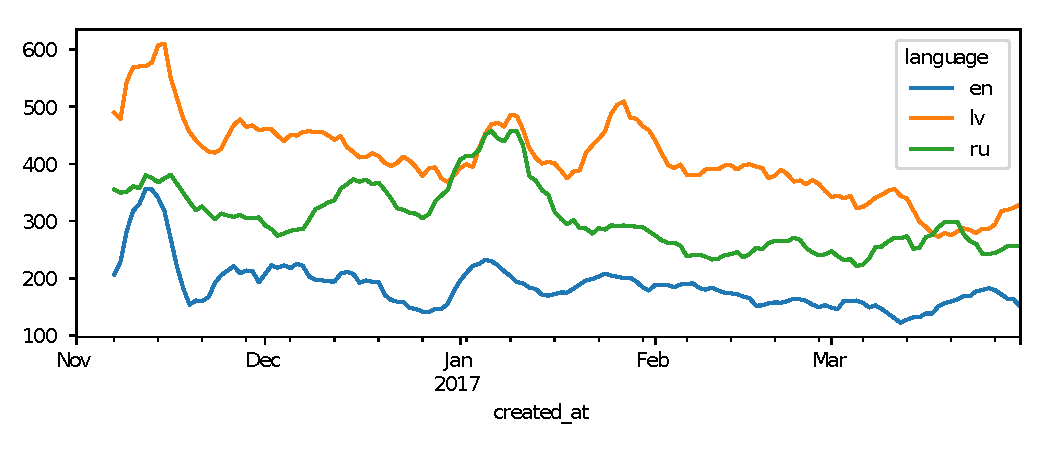
\includegraphics[width=\textwidth]{supplement/figures/timeline.pdf}
\caption{Tweet counts per day per language. The values are averaged over a week
  window at the right edge.}
\label{fig:timeline}
\end{figure*}

Out of 136\,067 tweets that constitute the final collection, 45.5\% are in Latvian, 33.9\% are in Russian and 20.7\% are in English, see Table~\ref{tab:language-counts} for tweet counts.
% The ratio between the Latvian and Russian tweets is roughly the same as the proportion of ethnic Latvians and Russians in Riga, which is 46.2\% to 37.7\%.\footnote{\url{https://en.wikipedia.org/wiki/Riga}}

\begin{table}[ht]
  \centering
  \small
  \begin{tabular}{lrrr}
    \toprule
    Language & Tweet count & Share \% & Avg. token count \\
    \midrule
    Latvian     & 61\,869  & 45.4\% & 15 \\
    Russian     & 46\,070  & 33.9\% & 11 \\
    English     & 28\,128  & 20.7\% & 14 \\
    \bottomrule
  \end{tabular}
  \caption{Language distribution in the final collection.}
  \label{tab:language-counts}
\end{table}

Figure~\ref{fig:timeline} shows the bandwidth of tweets over time for all three languages. There are several peaks in Twitter usage. Some of them affect all three languages, as in early January, some of them affect only one language, as in late January. % Any significance? Ah, I see next paragraph.

If the Twitter behaviour is affected by the events in the real world, then the peaks should correspond to events in the real word. The difference in peaks could then be explained as there are different real word events that trigger discussions on Twitter in Latvian, Russian and English. Table~\ref{tab:timeline-lang-corr} suggests, that tweets in Latvian and English share similar behaviour. The Russian tweet timeline is distinct from both timelines, tough its behaviour is more similar to the Latvian timeline than to English.

\begin{table}[ht]
  \centering

  \begin{tabular}{lrrr}
\toprule
Language &     Latvian & Russian & English \\
\midrule
Latvian       &  1.0 &  0.4 &  0.6 \\
Russian       &  0.4 &  1.0 &  0.3 \\
English       &  0.6 &  0.3 &  1.0 \\
\bottomrule
\end{tabular}

  
  \caption{Pairwise Pearson's-$\rho$ correlation coefficients between Latvian,
    Russian and English timelines.}
  \label{tab:timeline-lang-corr}
\end{table}

What are the distinctive and similar properties of the timelines? To answer the question, we first identify the real world events that happened during the biggest peaks.

\paragraph{Mid November}

11th of November is \href{https://en.wikipedia.org/wiki/L\%C4\%81\%C4\%8Dpl\%C4\%93sis_Day}{L\={a}\v{c}pl\={e}sis Day}, a memorial day for soldiers who fought for the independence of Latvia. 18 November is the Proclamation Day of the Republic of Latvia. Numerous events take place across the country including candle placing on and by the wall of Riga Castle, torchlight processions and fireworks. The volume of tweets peaks in all three languages, though the peak in Russian is less significant than in Latvian and English.

% \paragraph{Mid December}

% There is a higher amount of Russian tweets, but Latvian and English tweet volume stays constant.

\paragraph{Early January}

There is a lot of activity during the New Year celebration for all three languages. Russian tweets peak the most almost reaching the same number of tweets as tweets in Latvian.

\paragraph{Late January}

\begin{figure*}[t]
\centering
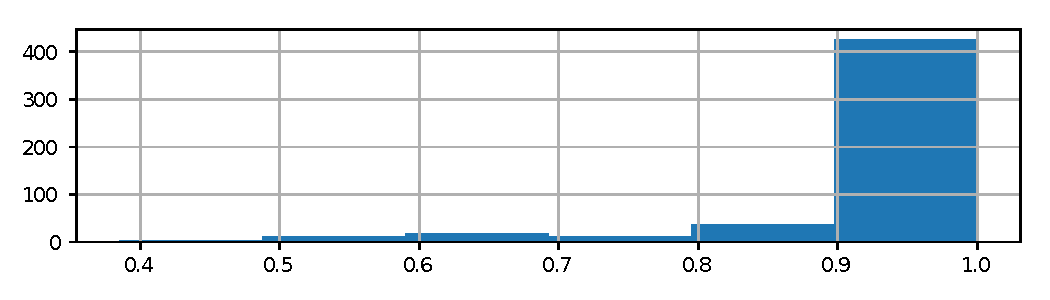
\includegraphics[width=\textwidth]{supplement/figures/score-hist.pdf}
\caption{Histogram of language use uniformity scores. Low values mean that
  distinct languages are used, while high values mean that a single language is preferred.}
\label{fig:score-hist}
\end{figure*}

The inauguration of Donald Trump as the 45th President of the United States held on 20th of January 2017. The number of Latvian tweets increases, while for other languages it stays roughly the same.

% \paragraph{Early March}

% There are peaks in Latvian and Russian tweets.

% \paragraph{Mid March}

% There is a general decline in Twitter usage for Latvian and English, but not for Russian, when for a short period of time there are more Russian tweets posted than Latvian.

Timeline analysis gives an insight of what events are reflected on Twitter, but does not indicate how Twitter is used by ethnic groups, as language choice might depend on the topic.

\section{User analysis}
\label{sec:lang-use}

We have seen that the reflection of an event on Twitter depends on the language. How are languages used individually? Do Twitter users tweet in one language all the time, or switch between languages depending on the context?

We consider 507 users for whom at least 50 tweets were collected. 180 or 35.5\% of them tweet exclusively in one language (75 users tweet only in Latvian, 43 in Russian and 62 in English). Others tweets in several languages.

To get more insight on how languages are used, we compute the language uniformity score defined as:
\begin{equation}
  \label{eq:score}
  \frac{\max(n_\mathit{lv}, n_\mathit{ru}, n_\mathit{en})}{n_\mathit{lv} + n_\mathit{ru} + n_\mathit{en}}
\end{equation}
where $n_\mathit{lv}$ corresponds to the number of tweets in Latvian for a given user, $n_\mathit{ru}$ in Russian and $n_\mathit{en}$ in English.

%The higher the score, the more dominant one language.
The lowest possible value of 0.33 means that all three languages are used equally. The value of 0.5 means that 50\% of tweets are written in a dominant language. The value of 1 means that the user tweets exclusively in one language.

The histogram on Figure~\ref{fig:score-hist} shows the score distribution. 420 (82.8\%) users tweet mostly in one language (their scores are greater than 0.9). For 83  (16.4\%) users the score is between 0.5 and 0.9. There are only four (0.8\%) users whose dominant language share is less than 50\%.

Among the four Twitter users whose score is less than 0.5---meaning that they use all three languages extensively---three are personal accounts and one is a company account. Another interesting accounts that tweet equally in Latvian and Russian, but do not tweet in English are the accounts of a library and a football club.

To illustrate the language usage pattern between multilingual users, their first most frequently used language, their second most frequently used language and their third most frequently language were identified. If user tweeted equally in two (three) languages, then the two (three) languages were given the maximal preference. A user who tweeted equally in Latvian and Russian, but less in English, will counted as Latvian and Russian being the first perference, English as the third.

Latvian is not only the most used language among the monoligual users, but also is the first and third most common choice between the multilingual users. The preference for Russian is similar to Latvian, despite the numbers being slightly lower, suggesting its significant role in everyday life. English is almost the ultimate second choice, proving its role as lingua franca, as Table~\ref{tab:language-use} shows.

\begin{table}[h]
  \centering
  \begin{tabular}{lrrr}
    \toprule
     & Latvian & Russian & English \\
    \midrule
    Monoligual     & \textbf{75} & 43 & 62  \\
    \addlinespace
    Multi, first   & \textbf{42} & 18 & 22  \\
    Multi, second  & \textbf{58} &  6 & 18  \\
    Multi, third   & 5  & \textbf{55} & 22  \\
    \bottomrule
  \end{tabular}
  \caption{Language choice between monolingual and multilingual users.}
  \label{tab:language-use}
\end{table}

\section{Conclusion}

We have seen that location-based tweet collection produces adequate results. Tweets in all three target languages were collected, and the resulted collection reflects real world events.

To produce reliable statistics, more data has to be collected. One way of getting more data (apart from a longer data collection period) is to retrieve tweets that contain words that are unique to a language \cite{sang2013}. This might work for Latvian, as it is reasonable to assume that a Latvian tweet originates from Latvia, but will not work for Russian and English.

Instead, the properties of this corpus might be used to bootstrap data collection. The most active users might be identified and their tweets collected. If having a balanced corpus is important, then multilingual users might be preferred over monolingual. The user connection graph might also be useful.

Regarding the social aspect of the corpus, the future work might have a look into why topics are language dependant? How separated/unified is the society? What are the controversial topics?

\bibliography{references,dmilajevs_publications}
\bibliographystyle{acl_natbib}

\end{document}
